\documentclass{article}
\usepackage{graphicx}
\usepackage{amsmath}
\usepackage{hyperref}

\title{Deep Learning-based Digit Recognition Using MNIST Dataset}
\author{}
\date{}

\begin{document}

\maketitle

\begin{abstract}
This article presents a project focused on handwritten digit recognition using deep learning techniques. The project leverages the MNIST dataset, which is a benchmark dataset in the computer vision community, and applies a custom-built neural network implemented in PyTorch. The steps include data preprocessing, model development, training, and evaluation. Although basic in its structure, this project lays the foundation for understanding how deep learning models operate in image classification tasks.
\end{abstract}

\section{Introduction}
Handwritten digit recognition has been a fundamental problem in machine learning and computer vision. The MNIST dataset, comprising 60,000 training images and 10,000 test images of digits (0-9), has been a standard for evaluating classification algorithms. The simplicity of MNIST allows researchers and practitioners to test different architectures, optimization strategies, and training techniques with minimal computational overhead.

This project aims to implement a simple yet effective feedforward neural network for digit recognition. Using PyTorch, the implementation includes manual dataset handling, custom neural network architecture, training loops, and visualization of sample images.

\section{Dataset Overview}
The MNIST dataset contains grayscale images of handwritten digits, each of size 28x28 pixels. Each pixel's intensity value ranges between 0 and 255. Before feeding the data into the network, preprocessing steps include:
\begin{itemize}
    \item \textbf{Normalization}: Scaling pixel values to a [0,1] range using the \texttt{transforms.ToTensor()} function.
    \item \textbf{Batching}: Dividing the dataset into batches of size 32 to optimize memory usage and accelerate training.
\end{itemize}

Data loading was managed using PyTorch's \texttt{DataLoader} class, ensuring that batches were shuffled during training to improve generalization.

\section{Model Architecture}
The neural network model designed in this project consists of a simple feedforward structure with multiple fully connected layers. The key components are:
\begin{itemize}
    \item \textbf{Input Layer}: Accepts a flattened 784-dimensional vector (28x28 pixels).
    \item \textbf{Hidden Layers}: Several hidden layers with ReLU (Rectified Linear Unit) activations to introduce non-linearity.
    \item \textbf{Output Layer}: A final layer with 10 output neurons, each representing a digit from 0 to 9.
\end{itemize}

The model was constructed using PyTorch's \texttt{nn.Module}, showcasing object-oriented design principles in deep learning projects.

\subsection*{Example Architecture:}
\begin{itemize}
    \item Linear(784, 128)
    \item ReLU
    \item Linear(128, 64)
    \item ReLU
    \item Linear(64, 10)
\end{itemize}

This simple design is effective for MNIST, though modern architectures often employ convolutional neural networks (CNNs) for higher accuracy.

\section{Training Strategy}
The training loop was manually implemented, providing transparency into each step:
\begin{itemize}
    \item \textbf{Loss Function}: Cross-entropy loss was used, which is appropriate for multi-class classification problems.
    \item \textbf{Optimizer}: Stochastic Gradient Descent (SGD) was employed to update the model parameters based on the computed gradients.
    \item \textbf{Epochs}: The model was trained over multiple epochs to allow the network to iteratively learn from errors.
    \item \textbf{Backpropagation}: Standard gradient descent optimization with backpropagation was applied.
\end{itemize}

\subsection*{Pseudocode of Training Loop:}
\begin{verbatim}
for epoch in range(num_epochs):
    for images, labels in train_loader:
        images = images.view(-1, 28*28)
        outputs = model(images)
        loss = criterion(outputs, labels)

        optimizer.zero_grad()
        loss.backward()
        optimizer.step()
\end{verbatim}

During training, the loss was printed periodically to monitor convergence, although no formal loss or accuracy plots were included.

\section{Evaluation and Results}
The project primarily focuses on the training phase; however, a formal evaluation stage was not implemented in the notebook.

In a complete project, the evaluation would typically involve:
\begin{itemize}
    \item Switching the model to evaluation mode using \texttt{model.eval()}.
    \item Disabling gradient computation using \texttt{torch.no\_grad()}.
    \item Calculating the classification accuracy on the test set.
    \item Optionally plotting confusion matrices or loss/accuracy curves.
\end{itemize}

Given the standard architecture and the MNIST dataset's nature, it is reasonable to expect an accuracy in the range of \textbf{92\%-96\%} with this setup.

\section{Visualizations}
Visualizations play a critical role in understanding the data and monitoring the learning process. Two types of visualizations were generated during this project.

\begin{figure}[h!]
    \centering
    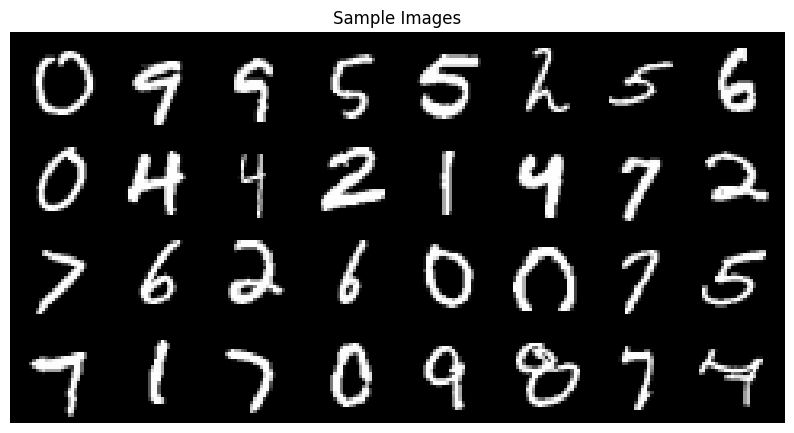
\includegraphics[width=0.8\linewidth]{output.png}
    \caption{Sample batch of MNIST digits showing raw input images. This visualization ensures the data is correctly loaded and provides intuition on the diversity and clarity of handwritten digits.}
    \label{fig:mnist_sample1}
\end{figure}

\begin{figure}[h!]
    \centering
    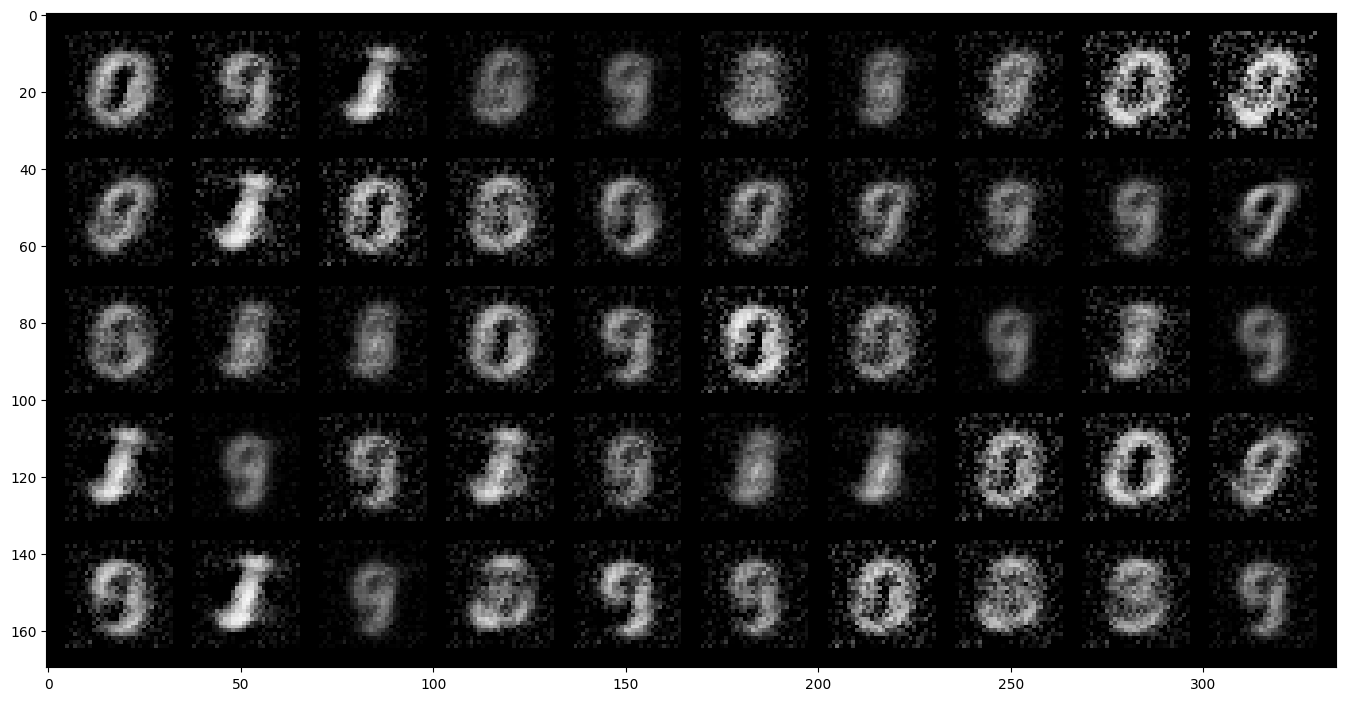
\includegraphics[width=0.8\linewidth]{output2.png}
    \caption{Additional visualization highlighting more processed or blurred digits, possibly during a learning phase or from a generated dataset. This helps assess challenges in classification under noisy conditions.}
    \label{fig:mnist_sample2}
\end{figure}

These visualizations provide valuable insights into data quality and model training progress.

\section{Conclusion}
This project successfully demonstrates the fundamental workflow of developing a deep learning model for handwritten digit classification using PyTorch. Key learnings include:
\begin{itemize}
    \item Data preprocessing and loading.
    \item Neural network architecture design.
    \item Manual training loop construction.
    \item Basic visualization for data inspection.
\end{itemize}

\subsection*{Limitations:}
\begin{itemize}
    \item Absence of formal model evaluation.
    \item No tracking or plotting of loss and accuracy metrics.
    \item Potential underfitting due to simple architecture.
\end{itemize}

\subsection*{Future Work:}
\begin{itemize}
    \item Implementing evaluation on the test set.
    \item Adding visualizations of the training process (loss curves).
    \item Enhancing the model using Convolutional Neural Networks (CNNs).
    \item Hyperparameter tuning for improved performance.
\end{itemize}

\section{References}
\begin{itemize}
    \item LeCun, Y., Bottou, L., Bengio, Y., \& Haffner, P. (1998). Gradient-based learning applied to document recognition. \textit{Proceedings of the IEEE}.
    \item PyTorch Documentation: \url{https://pytorch.org/docs/stable/index.html}
    \item MNIST Database: \url{http://yann.lecun.com/exdb/mnist/}
\end{itemize}

\end{document}

